
\section{Introduction}

Large language models (LLMs) have rapidly saturated many static benchmarks, leaving limited headroom for single-turn QA and reasoning datasets such as AIME~\citep{aime2024}, SWE-Bench~\citep{jimenez2023swe}, and GPQA~\citep{rein2024gpqa}. This shifts attention toward multi-turn and interactive evaluations, namely game-based benchmarks~\citep{duan2024gtbench,topsakal2024evaluating,fan2024can}, which stress long-horizon reasoning, adaptation, and strategic interaction. Games are easy to simulate, come with objectives, and require capabilities that apply to real-world challenges such as planning under uncertainty, negotiation, and context-sensitive decision making.

However, \emph{multi-turn, multi-agent LLM evaluation is inherently unstable}. Because each model output becomes part of the subsequent input, small early deviations can compound across turns, leading to divergent trajectories~\citep{laban2025llms}. In multi-agent games, interaction coupling can worsen this effect. An inconsistent response from one agent can perturb the other agent's best responses, reshaping the joint trajectory~\citep{cemri2025multi}. Separately, some LLMs exhibit nondeterministic outputs even under nominally deterministic decoding settings~\citep{blair2025llms}. From an evaluation perspective, these factors can bias win-rate estimates and destabilize comparative rankings across repeated tournaments, complicating reproducibility and fair model comparison.

Inference-time \emph{context}, including prompts, instructions, and auxiliary information, offers a direct lever for performance in interactive settings. Small contextual variations can induce different effective policies and rank reversals across models (Appx.~\ref{appendix:prompt_sensitivity}), motivating treatment of context not as a fixed wrapper but as an \emph{agentic object} that should be optimized under interaction.

Existing approaches, however, struggle in multi-turn, path-dependent games. Prompt engineering techniques such as chain-of-thought (CoT)~\citep{wei2022chain} instructions or hand-designed templates remain fixed throughout evaluation. While these can improve win rate or reduce superficial errors, they do not adapt to failure modes or strategic patterns that emerge through interaction. Automatic prompt optimization methods~\citep{yuksekgonul2024textgrad,yin2025llm,agrawal2025gepa,opsahl2024optimizing} allow prompts to adapt, but are largely developed for static tasks. They update prompts using feedback from a local batch of trajectories and lack persistent memory. In multi-turn, multi-agent games, different tournaments surface different decisive states and rare failure modes; without a mechanism to retain and reuse insights across rounds, prompt optimization becomes run-dependent, leading to high variance in both learned contexts and performance.

We therefore propose \textbf{MEMO} (\textbf{Me}mory-augmented \textbf{MO}del context optimization), a self-play framework that optimizes inference-time context without updating model weights. MEMO couples \emph{exploration}, tournament-style context evolution with uncertainty-aware selection via \textsc{TrueSkill} and prioritized replay, with \emph{retention}, a persistent memory bank that distills self-play trajectories into structured insights through create, read, update, and delete (CRUD) style operations and reinjects them as priors in subsequent rounds. The central finding is that exploration alone yields only modest gains; persistent memory is what transforms context optimization from a memoryless search into a cumulative learning process.

Across five text-based games from \texttt{TextArena} and \texttt{SPIN-Bench}~\citep{guertler2025textarena,yao2025spin}, \NAME{} raises mean win rate from \textbf{25.1\%} to \textbf{49.5\%} for \textbf{GPT-4o-mini}~\citep{openai2024gpt4o_mini} and from \textbf{20.9\%} to \textbf{44.3\%} for \textbf{Qwen-2.5-7B-Instruct}~\citep{yang2025qwen2_5}. It uses only 2{,}000 self-play games per task, 19$\times$ fewer than RL baselines, while reducing run-to-run variance by 7$\times$ to a relative standard error of 6.4\% compared to 43.3\%.

% \needspace{8\baselineskip}%
We make three main contributions.
\begin{itemize}[leftmargin=1.5em, labelindent=0pt, labelsep=0.5em,topsep=1pt, itemsep=1pt]

  \item \textbf{Context sensitivity in multi-turn, multi-agent LLM games.}
  We show that evaluation outcomes are sensitive to context choices. 
  Small prompt variations can shift effective policies and alter model rankings, motivating robust practices such as prompt-variation reporting rather than reliance on single-prompt evaluations.

  \item \textbf{A unified framework of reflection, memory, and replay.}
  We introduce a framework that combines structured reflection, persistent memory, context evolution, and prioritized replay, allowing the agent to accumulate and reuse knowledge across rounds rather than discarding it at each update.

  \item \textbf{Training-efficiency gains with improved stability.}
  We report that MEMO substantially improves win rates under a fixed self-play budget while reducing run-to-run variance of end-to-end outcomes.
  It achieves competitive or stronger results than existing prompt optimization methods in imperfect information games, while RL remains more effective in perfect-information settings.
\end{itemize}


\begin{figure*}[t]
    \centering
    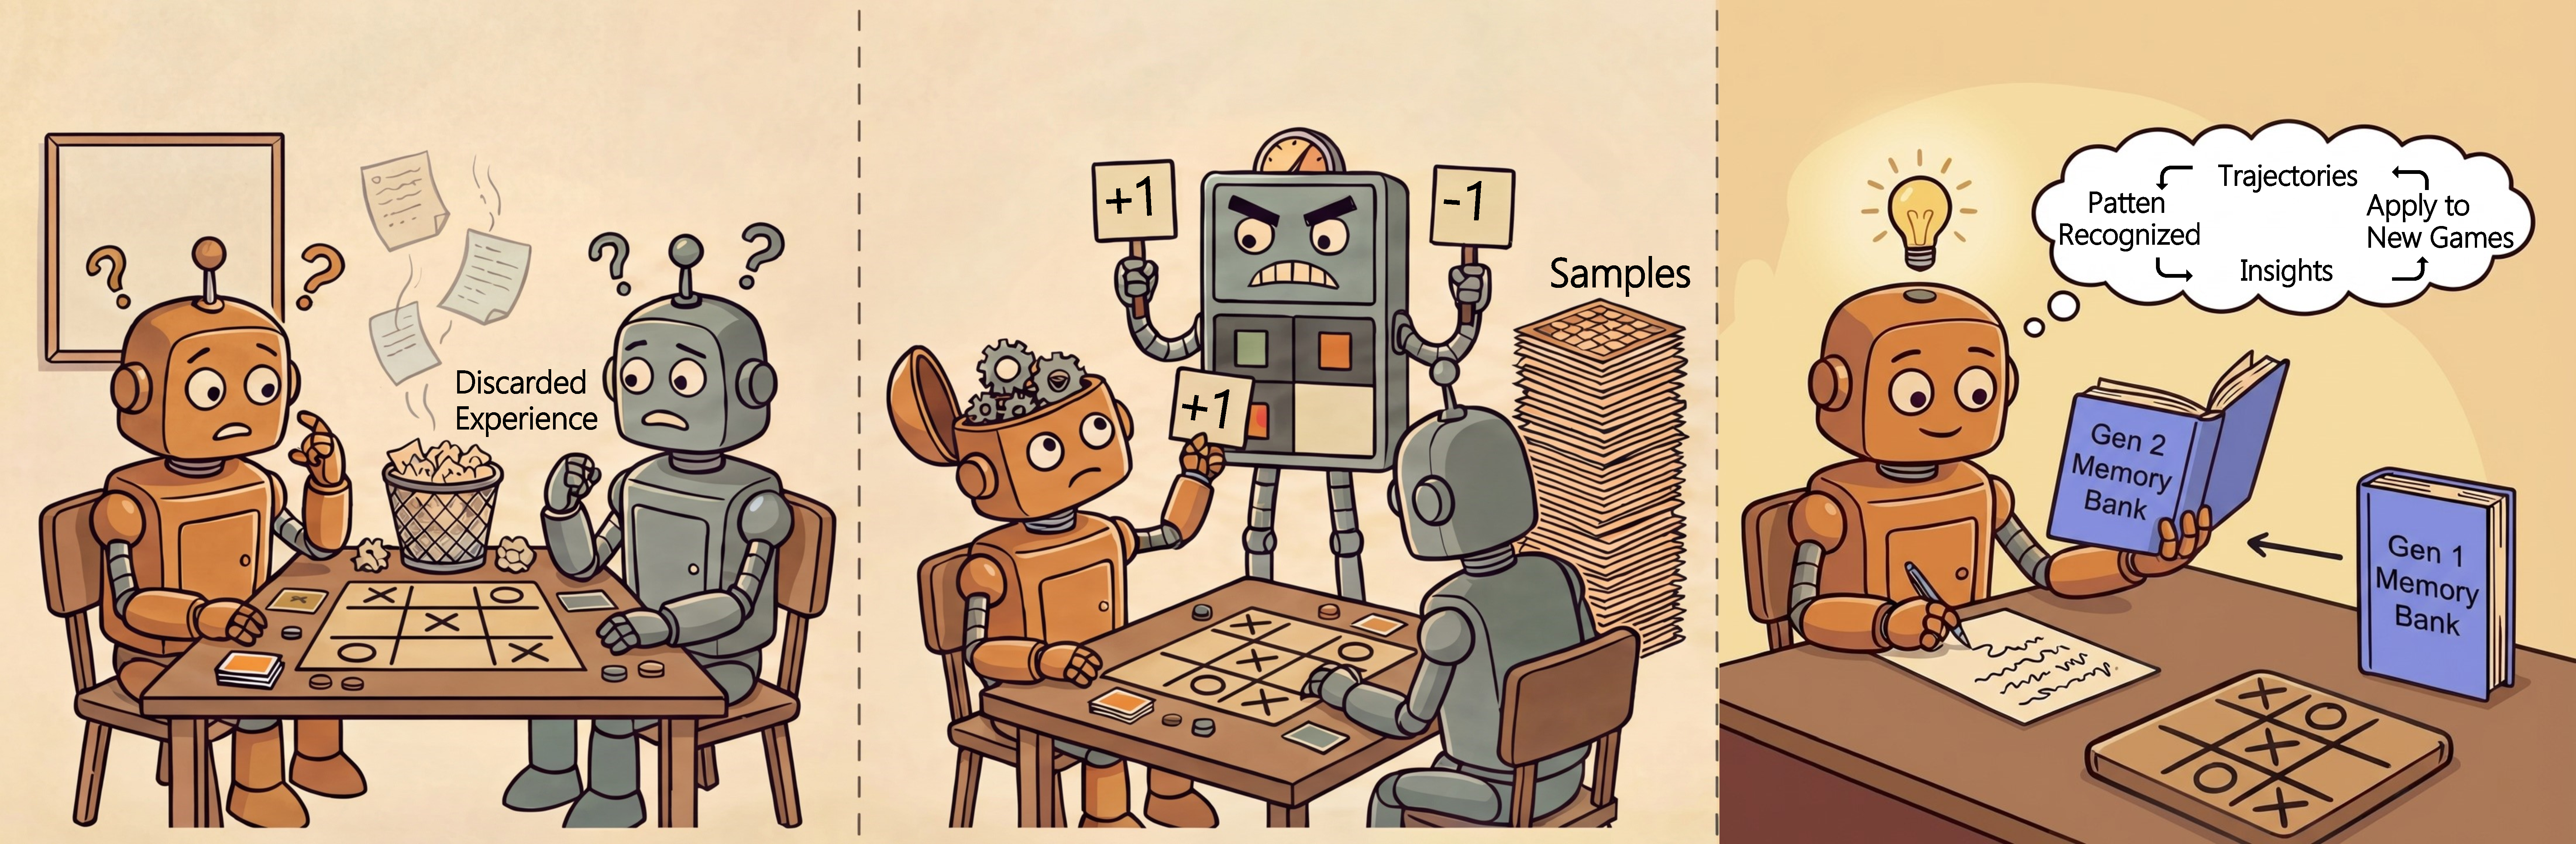
\includegraphics[width=\textwidth]{figures/comparison_visual.pdf}\\[2pt]
    \makebox[0.333\textwidth]{\small\textbf{(a) Self-Play Prompt Optimization}}%
    \makebox[0.333\textwidth]{\small\textbf{(b) Reinforcement Learning}}%
    \makebox[0.333\textwidth]{\small\textbf{(c) \NAME{} (Ours)}}
    \caption{\textbf{Three paradigms for learning in multi-agent LLM games.}
    \textbf{(a)}~Prompt optimization updates the system prompt each round
    through self-play, but game experience is not effectively retained across rounds,
    so strategic insights are lost across rounds.
    \textbf{(b)}~Reinforcement learning (RL) updates model weights through
    self-play but relies on outcome rewards, requiring large sample budgets.
    \textbf{(c)}~\NAME{} reflects on completed trajectories and accumulates
    reusable insights in a persistent memory bank across generations,
    enabling improvement without weight updates or external reward.}
    \label{fig:conceptual}
\end{figure*}

